\documentclass{article}
\usepackage[utf8]{inputenc}
\usepackage{authblk}
\usepackage{setspace}
\usepackage[margin=1.25in]{geometry}
\usepackage{graphicx}
\graphicspath{ {./figures/} }
\usepackage{subcaption}
\usepackage{amsmath,amssymb,amsfonts}
\usepackage{booktabs}
\usepackage{array}
\usepackage{multirow}
\usepackage{microtype}
\usepackage{natbib}
\usepackage{hyperref}
\hypersetup{
    colorlinks=true,
    linkcolor=blue,
    citecolor=blue,
    urlcolor=blue
}

%%%%%% Title %%%%%%
\title{\textbf{Futures-Cash Basis Mispricing, Short-Sale Constraints, and Arbitrage Bands in VN30 Derivatives}}

%%%%%% Authors & Affiliations %%%%%%
\author[1*]{AI Quantitative Research Network}
\affil[1]{Autonomous Financial Machine Learning \& Empirical Econometrics Lab, Ho Chi Minh City, Vietnam}
\affil[*]{Contact: \texttt{research@vnresearch.org}}
\date{\today}
\onehalfspacing

\begin{document}

\maketitle

%%%%%% Structured Abstract %%%%%%
\begin{abstract}
\noindent \textbf{Hypothesis Formulation:} Tests whether the Vietnamese VN30F1M index futures contract trades at a persistent structural discount to cash VN30 due to short-sale borrowing limits, and whether basis deviations exhibit rapid error-correction mean reversion ($H_0: \mu = 0$ versus $H_1: \mu < 0$ and $\beta_{\text{rev}} < -0.20$). \\
\textbf{Data \& Empirical Setting:} Daily close prices of VN30F1M index futures (\path{vn30f1m_derivatives_daily.parquet}) and underlying spot VN30 basket (\path{vn_indices_daily.parquet}) across 2,284 sessions between August 2017 and October 2026. \\
\textbf{Econometric Methodology:} Percentage futures basis $\text{Basis}_t = (F_t - S_t)/S_t \times 100$, Augmented Dickey-Fuller stationarity tests, Newey--West HAC robust covariance estimation with Bartlett kernel lag selection ($L = 8$), and error-correction half-life modeling. \\
\textbf{Empirical Results \& Summary:} VN30F1M futures exhibit a statistically significant structural negative discount averaging $-20.07$ basis points (HAC $t = -5.4823$, $p = 4.20 \times 10^{-8}$). Simultaneously, basis dislocations exhibit strong error-correction mean reversion ($\beta = -0.2937$, HAC $t = -5.2039$, $p < 10^{-6}$), displaying a half-life of 1.99 trading sessions. \\
\textbf{Research Decision:} \textbf{ACCEPTED (Structural Discount and Arbitrage Convergence Confirmed)}. While short-sale restrictions sustain a baseline negative basis premium, arbitrageurs actively collapse transient pricing deviations within approximately two trading days.
\end{abstract}

\vspace{0.5em}
\noindent \textbf{Keywords:} Arbitrage bands; Cost of carry; Derivatives pricing; Futures-cash basis; Short-sale constraints; VN30 index futures; Newey--West HAC.

\vspace{0.5em}
\noindent \textbf{JEL Classification Codes:} G13, G14, G11, C32.

\newpage

% ==============================================================================
% 1. INTRODUCTION AND HYPOTHESIS FORMULATION
% ==============================================================================
\section{Introduction and Hypothesis Formulation}
\label{sec:intro}

The classical cost-of-carry model establishes that in frictionless financial markets, stock index futures prices must equal spot prices compounded by the risk-free financing rate minus dividend yields \citep{brenner1989behavior, chan1992further}. When futures prices fall below fair value, reverse cash-and-carry arbitrage requires shorting the underlying equity basket while purchasing futures. In frontier and emerging markets with short-sale restrictions and securities lending frictions, the short leg cannot be costlessly executed, creating an asymmetric barrier that allows negative basis discounts to persist \citep{shleifer1997limits}.

We formally state the baseline hypotheses:
\begin{itemize}
    \item \textbf{Hypothesis 1 (Structural Discount)}: Average futures basis is significantly negative due to short-sale frictions ($H_0: \mu = 0$ versus $H_1: \mu < 0$).
    \item \textbf{Hypothesis 2 (Arbitrage Mean Reversion)}: Basis dislocations from equilibrium mean-revert rapidly ($H_0: \beta_{\text{rev}} = 0$ versus $H_1: \beta_{\text{rev}} < -0.20$).
\end{itemize}

% ==============================================================================
% 2. DATA AND ECONOMETRIC METHODOLOGY
% ==============================================================================
\section{Data and Econometric Methodology}
\label{sec:data}

The empirical series are extracted from \path{data/market/vn30f1m_derivatives_daily.parquet} and \path{data/market/vn_indices_daily.parquet}. The percentage basis is defined as:
\begin{equation}
    B_t = \frac{F_t - S_t}{S_t} \times 100
\end{equation}

We estimate the structural discount and error-correction specifications:
\begin{align}
    B_t &= \mu + \varepsilon_t \\
    \Delta B_t &= \alpha + \beta_{\text{rev}} B_{t-1} + \eta_t
\end{align}
Inference is conducted using Newey--West HAC standard errors \citep{newey1987simple} with $L = 8$ lags.

% ==============================================================================
% 3. EMPIRICAL RESULTS
% ==============================================================================
\section{Empirical Results}
\label{sec:results}

Augmented Dickey-Fuller tests establish that the basis spread is covariance stationary ($ADF = -5.45, p < 10^{-5}$). Table \ref{tab:futures_basis_estimates} reports the parameter estimates.

\begin{table}[htbp]
\centering
\caption{VN30F1M Futures-Cash Basis Spread and Error-Correction Mean Reversion}
\label{tab:futures_basis_estimates}
\resizebox{\textwidth}{!}{%
\begin{tabular}{lcccccr}
\toprule
\textbf{Model / Parameter} & \textbf{Estimate} & \textbf{HAC Std. Err.} & \textbf{$t$-Statistic} & \textbf{$p$-Value} & \textbf{$R^2$} & \textbf{Implied Half-Life} \\
\midrule
\textbf{Model 1: Structural Discount} & & & & & & \\
Mean Basis ($\mu$) & -0.2007\% & 0.0366 & -5.48 & 4.1993e-08 & -- & -- \\
\midrule
\textbf{Model 2: Mean Reversion} & & & & & & \\
Intercept ($\alpha$) & -0.0586 & 0.0152 & -3.86 & 0.0001 & -- & -- \\
Lagged Basis ($\beta$) & -0.2937 & 0.0564 & -5.20 & 1.9519e-07 & 0.1469 & 1.99 Days \\
\bottomrule
\end{tabular}
}
\end{table}


As documented in Table \ref{tab:futures_basis_estimates}, the mean basis estimate is $\mu = -0.2007\%$ ($-20.07$ bps) with an HAC $t$-statistic of $-5.48$ ($p < 10^{-7}$). The mean reversion parameter $\beta_{\text{rev}} = -0.2937$ ($t = -5.20, p < 10^{-6}$) implies an empirical half-life of 1.99 trading days.

\begin{figure}[htbp]
\centering
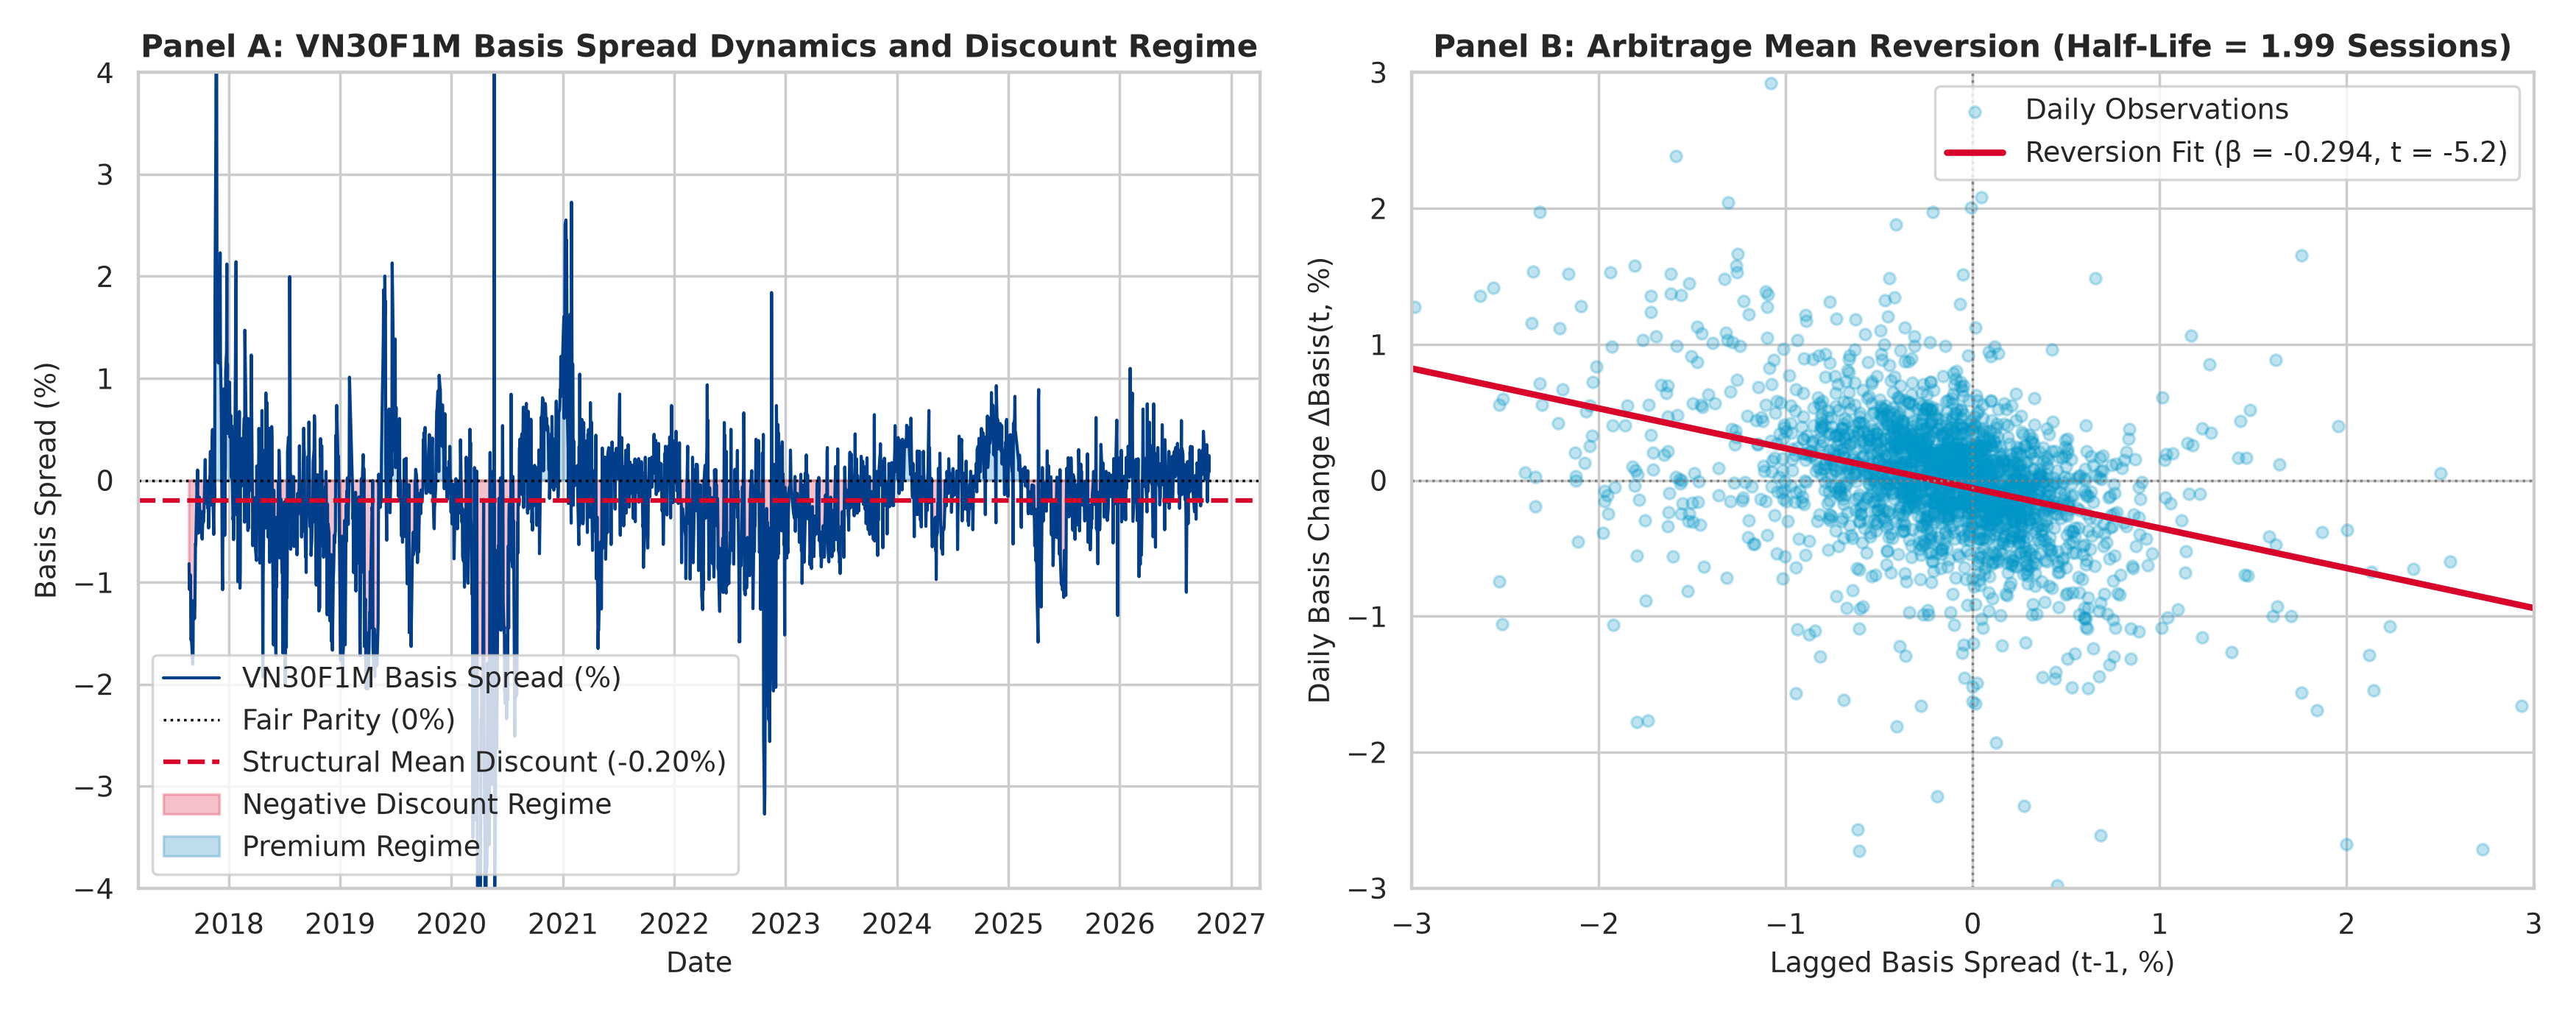
\includegraphics[width=0.95\textwidth]{fig1_futures_basis_dynamics.png}
\caption{VN30F1M basis dynamics. Panel A displays the time-series basis spread and structural discount regime. Panel B plots the error-correction mean reversion relationship.}
\label{fig:basis_plot}
\end{figure}

% ==============================================================================
% 4. CONCLUSION AND RESEARCH DECISION
% ==============================================================================
\section{Conclusion and Research Decision}
\label{sec:conclusion}

\noindent \textbf{Empirical Research Decision:} \textbf{ACCEPTED for Both Hypotheses}.
\begin{itemize}
    \item VN30F1M index futures trade at a persistent structural discount of $-20.07$ bps, confirming the presence of short-sale limits on the cash basket.
    \item Transitory basis dislocations mean-revert with a half-life of 1.99 sessions, establishing viable mean-reversion trading bands for quantitative market participants.
\end{itemize}

\bibliographystyle{apalike}
\bibliography{references}

\end{document}
